%!TEX ROOT = thesis.tex
\chapter{METHODOLOGY}

The implementation of this project is split into five different steps namely Data Collection, Data Preprocessing, Model Design and Implementation, Model Evaluation and Model Refinement.

\section{Data Collection}

There were 12 different datasets considered at the beginning of this project and their details can be found in Chapter 2. In the end, we decided to choose LoveDA dataset \ref{loveda} because of several reasons. The first reason is it has one of the lowest spatial resolution with 0.3m. The secondd reason is it has a total of 5,987 samples which I considered as a good number of samples. Te third reason is the images in LoveDA dataset is actually collected satellites unlike severeal other dataset that is a mixed of images collected therough satellites and drones. The final reason is the images on LoveDA comes in PNG format which is much easier to work with compared to some other dataset that comes in GeoTIFF format. Although GeoTIFF carry more information, I concluded that thetime and effort reuired to preprocess and train models using GeoTIFF format is too much.

\section{Data Preprocessing}

The images in LoveDA dataset aare separated into two groups; the rural images and the urban images. Each of the group is already splitted into a training set, a validation set and a testing set.

\FloatBarrier
\begin{figure}[!h]
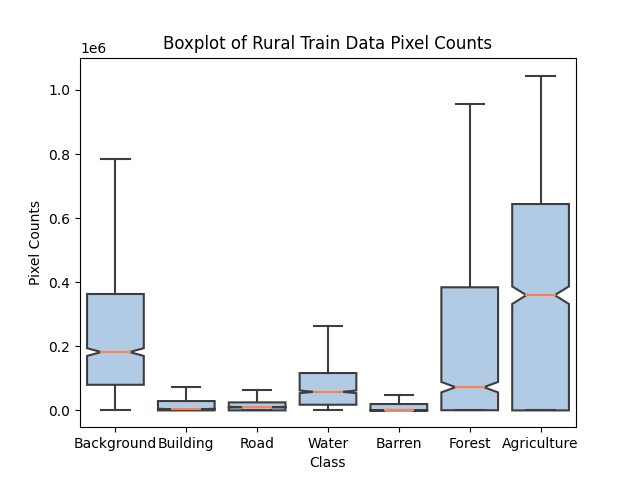
\includegraphics[width=15.0cm, height=8.5cm]{images/rural train boxplot.png}
\centering
\caption{Boxplot of the Pixel Counts of the Rural Train Dataset}
\label{fig:boxplot-rural-train}
\end{figure}

\begin{figure}[!h]
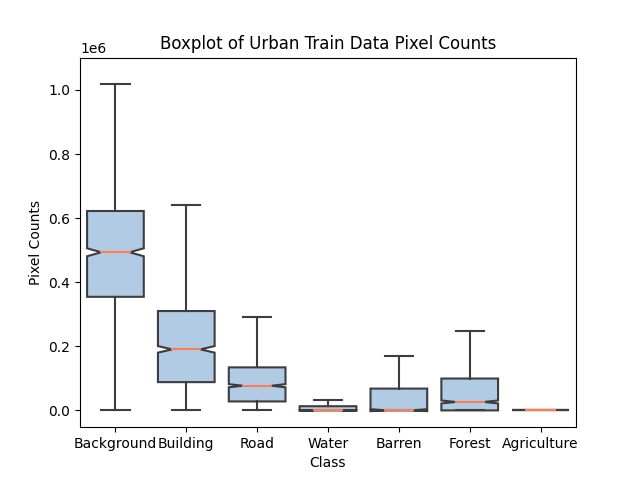
\includegraphics[width=15.0cm, height=8.5cm]{images/urban train boxplot.png}
\centering
\caption{Boxplot of the Pixel Counts of the Urban Train Dataset}
\label{fig:boxplot-urban-train}
\end{figure}

\begin{figure}[!h]
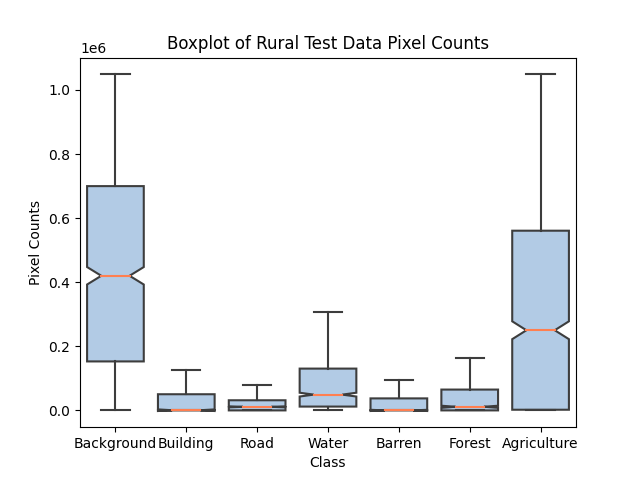
\includegraphics[width=15.0cm, height=8.5cm]{images/rural test boxplot.png}
\centering
\caption{Boxplot of the Pixel Counts of the Rural Test Dataset}
\label{fig:boxplot-rural-train}
\end{figure}

\begin{figure}[!h]
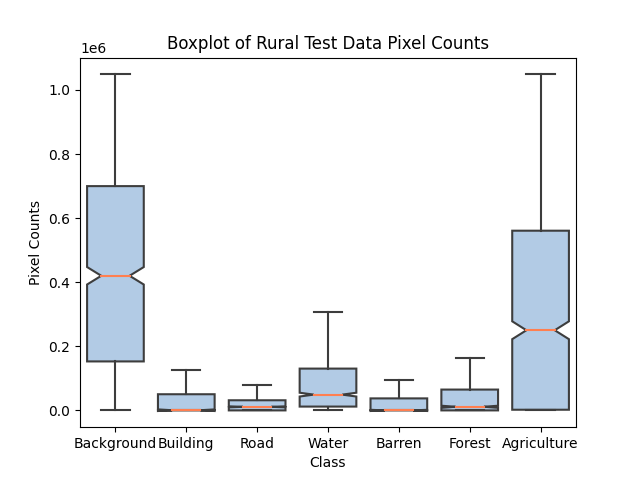
\includegraphics[width=15.0cm, height=8.5cm]{images/rural test boxplot.png}
\centering
\caption{Boxplot of the Pixel Counts of the Urban Test Dataset}
\label{fig:boxplot-urban-train}
\end{figure}
\FloatBarrier






\section{Model Design and Implementation}

\section{Model Evaluation}

\section{Model Refinement}
